%
\begin{isabellebody}%
\setisabellecontext{paper{\isadigit{3}}{\isadigit{3}}}%
%
\isadelimtheory
%
\endisadelimtheory
%
\isatagtheory
%
\endisatagtheory
{\isafoldtheory}%
%
\isadelimtheory
%
\endisadelimtheory
%
\isadelimdocument
%
\endisadelimdocument
%
\isatagdocument
%
\isamarkupsubsection{Lessons Learned and Goals for Chapter 3%
}
\isamarkuptrue%
%
\endisatagdocument
{\isafolddocument}%
%
\isadelimdocument
%
\endisadelimdocument
%
\begin{isamarkuptext}%
In this chapter, I tested two prior attempts to formalize the Formula of Universal Law and found 
that these attempts didn't faithfully interpret the FUL. Specifically, certain properties that 
we expect to hold of the FUL didn't hold in these implementations. In an attempt to remedy these 
shortcomings, in the next chapter, I present my own custom implementation of the FUL that satisfies these properties
and is thus more faithful to the literature. Before presenting my 
implementation, I define some goals for my custom formalization based on learnings from prior
attempts and from philosophical literature on the FUL.

The results presented below are summarized in Figure \ref{fig:goalstable}. For each goal, I indicate which 
interpretations successfully meet that goal. The fact that my custom formalization meets all the goals
indicates that it improves on prior formalization attempts. Below I will explain and justify
the goals.%
\end{isamarkuptext}\isamarkuptrue%
%
\begin{figure}
\centering
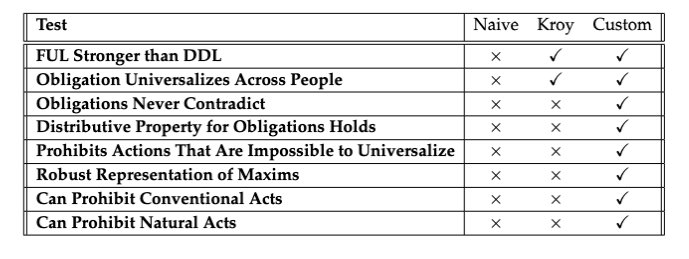
\includegraphics[scale=0.4]{goalstable.png}
\caption{Table indicating which goals are met by the naive formalization, Kroy's formalization, and 
the custom formalization respectively.} \label{fig:goalstable}
\end{figure}
%
\isadelimdocument
%
\endisadelimdocument
%
\isatagdocument
%
\isamarkupsubsubsection{Goals From Prior Attempts \label{sec:priorgoals}%
}
\isamarkuptrue%
%
\endisatagdocument
{\isafolddocument}%
%
\isadelimdocument
%
\endisadelimdocument
%
\begin{isamarkuptext}%
\textbf{FUL Stronger than DDL} One simple objective that the naive formalization failed to meet is the fact that the FUL should
not hold in the base logic (DDL). Recall that the naive formalization of the FUL\footnote{
This formalization reads $\vDash ((\neg (\square P \{A\})) \longrightarrow O \{\neg A\})$.} held in the 
base logic, so adding it as an axiom didn't make the logic any stronger. This is troubling 
because the base logic does not come equipped with the categorical imperative built-in. It 
defines basic properties of obligation, such as ought implies can, but contains no axioms that represent
the formula of universal law. Therefore, if a formalization of the FUL holds in the 
base logic, then it is too weak to actually represent the FUL. The naive interpretation holds in DDL but Kroy's formalization
does not. Because the naive interpretation is no stronger than DDL, it is acts a control group equivalent
to DDL itself.

\medskip 

\textbf{Obligation Universalizes Across People} Another property of the Formula of Universal Law that any implementation should satisfy is that obligation
generalizes across people. In other words, if a maxim is obligated for one person, it is obligated
for all other people because maxims are not person-specific. Velleman argues that, because 
reason is accessible to everyone identically, obligations apply to all people equually \cite[25]{velleman}. 
When Kant describes the categorical imperative as the objective principle of the will, he is referring 
to the fact that, as opposed to a subjective principle, the categorical imperative applies to all 
rational agents equally \cite[16]{groundwork}. At its core, the FUL best handles, ``the temptation 
to make oneself an exception: selfishness, meanness, advantagetaking, and disregard for the rights 
of others" \cite[30]{KorsgaardFUL}. Kroy latches onto this property and makes it the content of his
formalization, which essentially says that if an act is permissible for someone, it is permissible for 
everyone.\footnote{Formally, $P\{A(s)\} \longrightarrow \forall p. P\{A(p)\}$} While Kroy's interpretation 
clearly satisfies this property, the naive interpretation does not.

\medskip

\textbf{Contradictory Obligations} Another problem with prior formalizations was that they didn't
prohibit contradictory obligations, partially because DDL itself allows contradictory obligations. 
Kant subscribes to the general, popular view that morality is supposed to guide action, so ought implies 
can.\footnote{Kohl points out that this principle is referred to as 
Kant's dictum or Kant's law in the literature \cite[footnote 1]{kohl}.} Kohl reconstructs his argument for the principle as 
follows: if the will cannot comply with the moral law, then the moral law has no prescriptive authority 
for the will \cite[703-4]{kohl}. This defeats the purpose of Kant's theory—to develop an unconditional, categorical imperative 
for rational agents. Ought implies can requires that obligations never contradict, because an agent 
can't perform contradictory actions. Therefore, any ethical theory that respects ought implies can, 
and Kantian ethics in particular, must not result in conflicting obligations. 
Kant only briefly discusses contradictory obligations in \emph{Metaphysics of Morals}, where he argues that 
conflicting moral obligations are impossible under his theory \cite[V224]{metaphysicsintro}. Particularly, the categorical imperative generates 
``strict negative laws of omission," which cannot conflict by definition \cite[45]{timmerman}. \footnote{The 
kinds of obligations generated by the FUL are called ``perfect duties" which arise from ``contradictions 
in conception," or maxims that we cannot even concieve of universalizing. These duties are always negative 
and thus never conflict. Kant also presents ``imperfect duties," generated from ``contradictions in will,"
or maxims that we can concieve of universalizing but would never want to. These duties tend to be broader, 
such as ``improve oneself" or "help others," and are secondary to perfect duties. My project only analyzes 
perfect duties, as these are always stronger than imperfect duties.}. Both the naive formalization and 
Kroy's formalization allow contradictory obligations. 

During testing, I also realized that contradictory obligations are closely related to two other properties
that also fail in both of these systems. First is the idea that obligation implies permissibility, or 
that obligation is a stronger property than permissibility. If there are no contradictory obligations, 
then this property holds because actions are either permissible or prohibited and obligation contradicts
prohibition. Moreover, in a system with contradictory obligations, this property fails because there is some
A that is obligated but also prohibited and therefore not permisible. Indeed, formalizing this property below shows 
that this follows from the definition of implication in propositional logic.

\medskip%
\end{isamarkuptext}\isamarkuptrue%
\isacommand{lemma}\isamarkupfalse%
\ {\isachardoublequoteopen}{\isasymTurnstile}\ {\isacharparenleft}{\isacharparenleft}O\ {\isacharbraceleft}A{\isacharbraceright}\ \isactrlbold {\isasymand}\ O\ {\isacharbraceleft}\isactrlbold {\isasymnot}\ A{\isacharbraceright}{\isacharparenright}\ \isactrlbold {\isasymequiv}\ {\isacharparenleft}\isactrlbold {\isasymnot}\ {\isacharparenleft}O\ {\isacharbraceleft}A{\isacharbraceright}\ \isactrlbold {\isasymrightarrow}\ \isactrlbold {\isasymnot}\ O\ {\isacharbraceleft}\isactrlbold {\isasymnot}A{\isacharbraceright}{\isacharparenright}{\isacharparenright}{\isacharparenright}{\isachardoublequoteclose}\isanewline
%
\isadelimproof
\ \ %
\endisadelimproof
%
\isatagproof
\isacommand{by}\isamarkupfalse%
\ simp%
\endisatagproof
{\isafoldproof}%
%
\isadelimproof
%
\endisadelimproof
%
\begin{isamarkuptext}%
\textbf{Distributive Property} Another property related to contradictory obligations is the distributive property for the obligation
operator.\footnote{Formally, $O\{A\} \wedge O\{B\} \longleftrightarrow O\{A \wedge B\}$.} This is 
another property that we expect to hold. The rough English translation of  $O \{ A \wedge B \} $ is ``you are obligated to 
do both A and B". The rough English translation of $O\{A\} \wedge O\{B\}$ is ``you are obligated to do A 
and you are obligated to do B." We think those English sentences mean the same thing, so they should mean 
the same thing in logic as well. Moreover, if that (rather intuitive) property holds, then contradictory
obligations are impossible, as shown in the below proof.%
\end{isamarkuptext}\isamarkuptrue%
\isacommand{lemma}\isamarkupfalse%
\ distributive{\isacharunderscore}implies{\isacharunderscore}no{\isacharunderscore}contradictions{\isacharcolon}\ \isanewline
\ \ \isakeyword{assumes}\ {\isachardoublequoteopen}{\isasymforall}A\ B{\isachardot}\ {\isasymTurnstile}\ {\isacharparenleft}{\isacharparenleft}O\ {\isacharbraceleft}A{\isacharbraceright}\ \isactrlbold {\isasymand}\ O\ {\isacharbraceleft}B{\isacharbraceright}{\isacharparenright}\ \isactrlbold {\isasymequiv}\ O\ {\isacharbraceleft}A\ \isactrlbold {\isasymand}\ B{\isacharbraceright}{\isacharparenright}{\isachardoublequoteclose}\isanewline
\ \ \isakeyword{shows}\ {\isachardoublequoteopen}{\isasymforall}A{\isachardot}\ {\isasymTurnstile}{\isacharparenleft}\ \isactrlbold {\isasymnot}{\isacharparenleft}O\ {\isacharbraceleft}A{\isacharbraceright}\ \isactrlbold {\isasymand}\ O\ {\isacharbraceleft}\isactrlbold {\isasymnot}\ A{\isacharbraceright}{\isacharparenright}{\isacharparenright}\ {\isachardoublequoteclose}\isanewline
%
\isadelimproof
\ \ %
\endisadelimproof
%
\isatagproof
\isacommand{using}\isamarkupfalse%
\ O{\isacharunderscore}diamond\ assms\ \isacommand{by}\isamarkupfalse%
\ blast%
\endisatagproof
{\isafoldproof}%
%
\isadelimproof
%
\endisadelimproof
%
\begin{isamarkuptext}%
Thus, while testing contradictory obligations, I also test the distributive property for the 
obligation operator. Again, this property fails in the naive formalization and for Kroy's formalization.


\medskip 

\textbf{Un-universalizable Actions} This goal is inspired by a test performed for Kroy's formalization. Under 
a naive reading of the Formula of Universal Law, it prohibits lying because, in a world 
where everyone simultaneously lies, lying is impossible. In other words, not everyone can simultaneously
lie because the institution of lying and believing would break down. More precisely, the FUL should 
show that actions that cannot possibly be universalized are prohibited, because those acts cannot be willed in 
a world where they are universalized. This property fails to hold in both the naive formalization 
and Kroy's formalization and is a goal for my custom formalization.%
\end{isamarkuptext}\isamarkuptrue%
%
\isadelimdocument
%
\endisadelimdocument
%
\isatagdocument
%
\isamarkupsubsubsection{Goals From Philosophical Literature \label{sec:litgoals}%
}
\isamarkuptrue%
%
\endisatagdocument
{\isafolddocument}%
%
\isadelimdocument
%
\endisadelimdocument
%
\begin{isamarkuptext}%
The goals above come from moral intuition, properties of Kantian ethics, and logical requirements. 
In order to stay faithful to centuries of philosophical debate about the meaning of the Formula of 
Universl Law, I also present some goals inpsired by this literature.

\textbf{Maxims} Kant does not evaluate the correctness of acts, but rather of maxims. Therefore, any 
faithful formalization of the categorical imperative must evaluate maxims, not acts. This requires 
representing a maxim and making it the input to the obligation operator, which neither of the prior attempts do.

\medskip%
\end{isamarkuptext}\isamarkuptrue%
%
\begin{isamarkuptext}%
\textbf{Conventional Acts}
Kantians debate over the most philosophically sound interpretation of the Formula of Universal Law.
One litmus test that Korsgaard introduces makes a distinction between conventional and natural acts \citep{KorsgaardFUL}. 
A conventional act is one like promising, which relies on the convention of promising, in which we all
implicitly understand a promise as a commitment. Conventional acts are generally easier to show the 
wrongness of because there are worlds in which these acts are impossible; namely, worlds in which the 
convention does not exist. For example, the common argument against falsely promising is that if 
everyone were to falsely promise, the convention of promising would fall apart because people wouldn't believe
each other anymore, so falsely promising is prohibited. Despite the relative ease of this property,
it fails in both the naive and Kroy's interpretations, demonstrating the weakness of these 
formalizations. This property will hold for my custom formalization.

\medskip 

\textbf{Natural Acts}
The more difficult kind of act to show the wrongness of is a natural act, like murder or violence. 
These acts can never be logically impossible; even if everyone murders or acts violently, murder and 
violence will still be possible. This property of natural acts makes it difficult for interpretations of
the FUL to show the wrongness of violence. Both the naive and Kroy's interpretations fail to show
the wrongness of natural acts (in fact, they fail to show the weaker wrongness of conventional acts). 
This property will hold for the custom formalization. I will show the wrongness of both natural and 
conventional acts by formalizing Korsgaard's practical contradiction interpretation of the FUL, which 
is widely accepted as the canonical interpretation of the FUL \citep{KorsgaardFUL}. I will explain this 
decision in greater detail in the next chapter, where I present my custom formalization.%
\end{isamarkuptext}\isamarkuptrue%
%
\isadelimtheory
%
\endisadelimtheory
%
\isatagtheory
%
\endisatagtheory
{\isafoldtheory}%
%
\isadelimtheory
%
\endisadelimtheory
%
\end{isabellebody}%
\endinput
%:%file=~/Desktop/cs91r/paper/paper33.thy%:%
%:%24=6%:%
%:%36=8%:%
%:%37=9%:%
%:%38=10%:%
%:%39=11%:%
%:%40=12%:%
%:%41=13%:%
%:%42=14%:%
%:%43=15%:%
%:%44=16%:%
%:%45=17%:%
%:%46=18%:%
%:%47=19%:%
%:%50=22%:%
%:%51=23%:%
%:%52=24%:%
%:%53=25%:%
%:%54=26%:%
%:%55=27%:%
%:%63=29%:%
%:%75=31%:%
%:%76=32%:%
%:%77=33%:%
%:%78=34%:%
%:%79=35%:%
%:%80=36%:%
%:%81=37%:%
%:%82=38%:%
%:%83=39%:%
%:%84=40%:%
%:%85=41%:%
%:%86=42%:%
%:%87=43%:%
%:%88=44%:%
%:%89=45%:%
%:%90=46%:%
%:%91=47%:%
%:%92=48%:%
%:%93=49%:%
%:%94=50%:%
%:%95=51%:%
%:%96=52%:%
%:%97=53%:%
%:%98=54%:%
%:%99=55%:%
%:%100=56%:%
%:%101=57%:%
%:%102=58%:%
%:%103=59%:%
%:%104=60%:%
%:%105=61%:%
%:%106=62%:%
%:%107=63%:%
%:%108=64%:%
%:%109=65%:%
%:%110=66%:%
%:%111=67%:%
%:%112=68%:%
%:%113=69%:%
%:%114=70%:%
%:%115=71%:%
%:%116=72%:%
%:%117=73%:%
%:%118=74%:%
%:%119=75%:%
%:%120=76%:%
%:%121=77%:%
%:%122=78%:%
%:%123=79%:%
%:%124=80%:%
%:%125=81%:%
%:%126=82%:%
%:%127=83%:%
%:%128=84%:%
%:%129=85%:%
%:%130=86%:%
%:%131=87%:%
%:%132=88%:%
%:%134=92%:%
%:%135=92%:%
%:%138=93%:%
%:%142=93%:%
%:%143=93%:%
%:%152=95%:%
%:%153=96%:%
%:%154=97%:%
%:%155=98%:%
%:%156=99%:%
%:%157=100%:%
%:%158=101%:%
%:%160=103%:%
%:%161=103%:%
%:%162=104%:%
%:%163=105%:%
%:%166=106%:%
%:%170=106%:%
%:%171=106%:%
%:%172=106%:%
%:%181=108%:%
%:%182=109%:%
%:%183=110%:%
%:%184=111%:%
%:%185=112%:%
%:%186=113%:%
%:%187=114%:%
%:%188=115%:%
%:%189=116%:%
%:%190=117%:%
%:%191=118%:%
%:%192=119%:%
%:%193=120%:%
%:%202=122%:%
%:%214=124%:%
%:%215=125%:%
%:%216=126%:%
%:%217=127%:%
%:%218=128%:%
%:%219=129%:%
%:%220=130%:%
%:%221=131%:%
%:%222=132%:%
%:%226=136%:%
%:%227=137%:%
%:%228=138%:%
%:%229=139%:%
%:%230=140%:%
%:%231=141%:%
%:%232=142%:%
%:%233=143%:%
%:%234=144%:%
%:%235=145%:%
%:%236=146%:%
%:%237=147%:%
%:%238=148%:%
%:%239=149%:%
%:%240=150%:%
%:%241=151%:%
%:%242=152%:%
%:%243=153%:%
%:%244=154%:%
%:%245=155%:%
%:%246=156%:%
%:%247=157%:%
%:%248=158%:%
%:%249=159%:%